\subsection{Ecuaciones en diferencias}

\begin{frame}
\frametitle{\subsecname}

Aquí es conveniente representar cualquier sucesión de números reales $(a_{n})_{n} $ como la función $f\colon\mathds{N}\rightarrow\mathds{R}$ definido por: \[ f(n)=a_{n},\quad\forall n\in\mathds{N}. \]

\begin{definition}
	Una \textbf{ecuación en diferencias} es una expresión de la forma:
		\begin{equation}\label{eq:diffeq}
			G\left(n,f(n),f\left(n+1\right),\ldots,f\left(n+k\right)\right)=0,\quad\forall n\in\mathds{N}.
		\end{equation}
\end{definition}

El \textbf{orden} de una ecuación en diferencias se halla mediante la diferencia entre los ``términos mayor'' y ``menor'' respectivamente. En~(2), es \alert{$n+k-n=k$}.%\eqref{eq:diffeq}

\begin{example}
	\begin{itemize}
		\item El \alert{orden} de $f\left(n+3\right)-f\left(n+1\right)-5f(n)=n$ es \alert{$3$}.
		\item El \alert{orden} de $f\left(n+3\right)-f\left(n+1\right)=n^{2}-3$ es \alert{$2$}.
	\end{itemize}
\end{example}
\end{frame}

\begin{frame}

\begin{definition}
	Una \textbf{ecuación en diferencias} se le llama \textbf{lineal}	  si puede expresarse de la siguiente forma:
	\begin{equation}\label{edl}
		a_{0}(n)f\left(n+k\right)+a_{1}(n)f\left(n+k-1\right)+\cdots+a_{k-1}(n)f\left(n+1\right)+a_{k}(n)f\left(n\right)=b\left(n\right), 
	\end{equation}
	donde $a_{k}(n)\neq0$.
\end{definition}

\begin{block}{Clasificación}
	\begin{table}[H]
		\centering
		\begin{tabular}{|c|c|}
		\hline
		\alert{NOMBRE} 								& \alert{CONDICIÓN}\\
		\hline
		Homogéneas(E.D.L.H)						& si $b(n)=0$.\\
		\hline
		Completas (E.D.L.C)						& si $b(n)\neq0$.\\
		\hline
		De coeficientes constantes		& $a_{i}(n)=a_{i}$, $\forall i$.\\
		\hline
		De coeficientes no constantes	& si $a_{i}(n)\neq a_{i}$ para algún $i$.\\
		\hline
		\end{tabular}
	\end{table}
\end{block}
\end{frame}

\subsubsection{Homogénea de coeficientes constantes}
\begin{frame}
\frametitle{\subsecname}
%\begin{definition}
	%La \textbf{solución} de~(2) a toda sucesión $\{f\left(0\right),f\left(1\right),\ldots,f(n),\ldots\}$ que la satisfaga, ahora se le llama \emph{solución general} de una E.D al conjunto de todas las soluciones que tendrán tanto parámetros como orden tenga la ecuación. La determinación de estos parámetros, a partir de unas condiciones iniciales, nos proporcionará las distintas soluciones particulares.
%\end{definition}

\begin{definition}
	Sea una \textbf{ecuación en diferencias lineal homogénea} de coeficientes constantes y de orden $k$, buscaremos soluciones del tipo $f(n)=r^{n}$,haciendo este cambio y simplificando tenemos:
	\begin{align*}
	r^{n}(a_{0}r^{k}+a_{1}r^{k-1}+\cdots+a_{k})&=0\\
	\Rightarrow (a_{0}r^{k}+a_{1}r^{k-1}+\cdots+a_{k})&=0,
	\end{align*}
	a la expresión anterior llamaremos \textbf{ecuación característica}.
\end{definition}

\begin{definition}
	Llamamos \textbf{solución} de una E.D. a toda sucesión $\{ f(1), \ldots, f(k) \}$ que la satisfaga.
\end{definition}

\begin{definition}
	Se le llama \textbf{solución general} de una E.D. al conjunto de todas las soluciones, que tendrá tantos parámetros como orden tenga la ecuaciónón
\end{definition}
\end{frame}

\begin{frame}
%es $f\left(n\right)=3n+c$.
%Si consideramos las condiciones iniciales, por ejemplo, $f(0)=2$, entonces $f(0)=3\times0+c=c$, por tanto $c=2$ y la solución particular es $f_{p}(n)=3n+2$.
%Es decir, la solución es la sucesión $f_{p}(n)=\left\{2,5,8,11,\ldots\right\}$.
%\end{example}

\begin{theorem}[De la existencia y la unicidad]
	Dada la ecuación (\ref{edl}) y dados $n$ números reales $k_{0}$, $k_{1}$, \ldots, $k_{n-1}$ existe una única solución que verifica \[ f\left(0\right)=k_{0},f\left(1\right)=k_{1},\ldots,f\left(n-1\right)=k_{n-1}. \]
\end{theorem}

\begin{theorem}
	Toda combinación lineal de soluciones de una ecuación en diferencias lineal homogénea de orden $n$ es también una solución.
\end{theorem}

\begin{theorem}
	Las soluciones de una ecuación en diferencia lineal de orden $n$ forman un espacio vectorial,cuya dimensión del espacio de soluciones de una ecuación en diferencias lineal de orden $k$ es $k$.
\end{theorem}
\end{frame}

\begin{frame}
\begin{block}{Raíces simples}
	Sean $r_{1}, r_{2},\ldots, r_{k}$ las $k$ raíces de la ecuación característica. Se definen entonces las funciones: \[ f_{j}(n)=r^{n}_{j},\quad j=1,\ldots,k. \] Entonces, $f_{1},\ldots,f_{k}$ es un sistema fundamental de soluciones, lo cual nos permite resolver la ecuación. % TODO: Cuál ecuación.
\end{block}

\begin{block}{Raíces múltiples}
	Sea $r$ una raíz de multiplicidad $m$ de la ecuación característica. Esta raíz proporciona $m$ soluciones diferentes del tipo: \[ f_{j}(n)=n^{j}r^{n},\quad j= 0,\ldots,m-1. \] Por tanto, pasarán a formar parte del sistema fundamental de soluciones las funciones $f_{0},\ldots,f_{m-1}$; esto es: \[ r^{n},nr^{n},n^{2}r^{n},\ldots,n^{m-1}r^{n}. \]
\end{block}
\end{frame}

\begin{frame}

\begin{example}
	Hallar la solución de \[ f(n+3)-7f(n+2)+15f(n+1)-9f(n)=0,\quad\forall n\in\mathds{N}, \] con las condiciones iniciales $f(0)=-1$,  $f(1)=2$ y $f(2)=17$.
\end{example}

\begin{example}[E.D.L.C]
	Hallar la solución de \[ f(n+1)-2f(n)=2^{n},\quad\forall n\in\mathds{N}, \] con la condición inicial $f(0)=-1$.
\end{example}
\end{frame}
%http://personal.us.es/pnadal/Informacion/leccion5ecdiferencias.pdf
%\begin{frame}
%	\begin{block}{Ecuaciones en diferencias de primer orden}
%	\end{block}
%	
%	\begin{block}{Ecuaciones en diferencias de segundo orden}
%	\end{block}
%\end{frame}


\subsubsection{Número de Catalan}

\begin{frame}
\frametitle{\subsecname}

\begin{minipage}{6cm}
	\begin{block}{Triangulación}
	Una triangulación de un polígono es una partición del mismo en triángulos disjuntos cuyos vértices coinciden con los vértices del polígono.
	\end{block}
\end{minipage}
\begin{minipage}{5cm}
	\begin{figure}
		\centering
		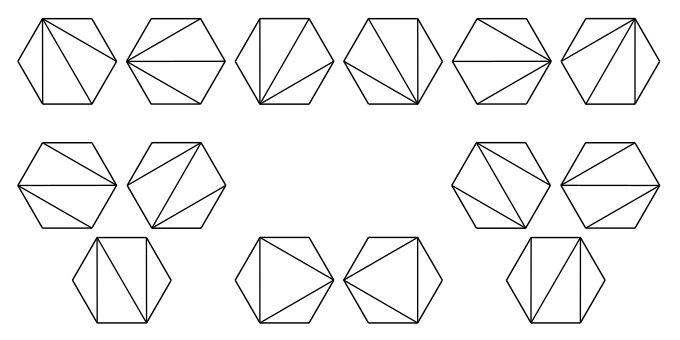
\includegraphics[scale=0.25]{ca1}	
	\end{figure}
\end{minipage}

\begin{minipage}{6cm}
	\begin{figure}
		\centering
		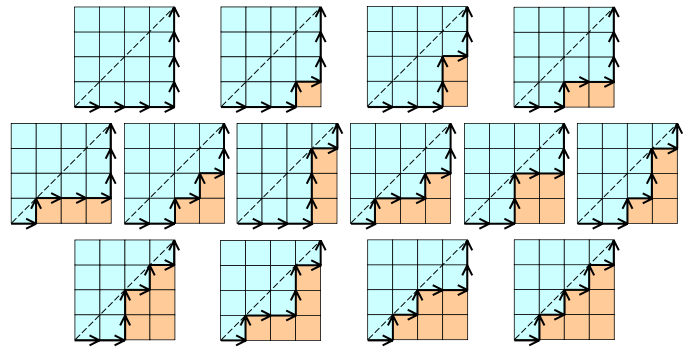
\includegraphics[height=0.3\paperheight]{ca(1)}
	\end{figure}
\end{minipage}
\begin{minipage}{5.5cm}
	\begin{block}{Caminos en rejillas}
		 Un camino monótono es aquél que empieza en la esquina inferior izquierda y termina en la esquina superior derecha, y consiste únicamente en tramos que apuntan hacia arriba o hacia la derecha,sin que pase de diagonal.
	\end{block}
\end{minipage}
\end{frame}